\documentclass[12pt,a4paper,utf8]{ctexart}
\usepackage{graphicx}
\usepackage{subfigure}
\usepackage{amsmath}
\usepackage{amssymb}
\usepackage{cases}
\usepackage{subfig}
\usepackage{cite}
\usepackage[ntheorem]{empheq}
\usepackage{enumitem}
\usepackage{fullpage}
\usepackage{cleveref}
\usepackage{cellspace}
\usepackage{listings}
\usepackage{color}

\usepackage{setspace}%使用间bai距宏包

\definecolor{gray}{rgb}{0.5,0.5,0.5}
\definecolor{dkgreen}{rgb}{.068,.578,.068}
\definecolor{dkpurple}{rgb}{.320,.064,.680}


% set Matlab styles
\lstset{
   language=Matlab,
   keywords={break,case,catch,continue,else,elseif,end,for,function,
      global,if,otherwise,persistent,return,switch,try,while},
   basicstyle=\ttfamily,
   keywordstyle=\color{blue}\bfseries,
   commentstyle=\color{dkgreen},
   stringstyle=\color{dkpurple},
   backgroundcolor=\color{white},
   tabsize=4,
   showspaces=false,
   showstringspaces=false,
   breaklines,%自动换行
   columns=fixed,
}

\begin{document}
\CJKfamily{zhkai}	


\begin{center}
    \begin{spacing}{2.0}%%行间距变为double-space
        \textbf{\heiti{\zihao {-1} 计算方法  作业二}}
     \end{spacing}
  
  \textbf{姓名 \quad 龚小航 \qquad  学号 \quad PB18151866  \qquad 日期\quad 2020.11.19}
\end{center}
\textit{}
\vspace{\baselineskip}

\begin{enumerate}
\item[第一题] 
  \begin{enumerate}
    \item[$a)$] 根据123页的算法,写出matlab程序。首先输出程序所支持的最大精度,由输出结果
                可知,最大精度约$10^{-16}$。因此在计算中将目标精度设为$tol=10^{-14}$。将
                最后一次迭代得到的结果作为计算误差的标准值。编写以下程序:
    \begin{lstlisting}[frame=single]
clear, clc
format long
%%用于求MATLAB能支持的最大精度
myeps = 1;
while 1~=(1+myeps)
myeps = myeps/2;
end
myeps = myeps*2
%%输出最大精度
%%利用课本123页的算法:
f = @(x) sin(cos(sin(cos(x))));  %积分函数
a = -1; b = 1;                   %积分区间[a,b]
tol = 1e-14;                     %误差控制精度
n = 1;                           %初始分点数
h = (b-a) / n;
iteration = 1;      %迭代次数
T2 = GETTN(a,b,n);  %初始n分点的复化梯形积分,T2 = Tn
TRES = zeros(100);  %记录每次迭代的结果,用于作图
TRES(iteration) = T2;
T1=T2+100;
%%while循环,参考课本算法
while abs(T1-T2)>tol   
    T1 = T2;
    H = h * sum(f(a + (2 * (1:n) - 1) * h / 2));
    T2 = (T1 + H) / 2;
    TRES(iteration) = T2;
    h = h / 2;
    n = n * 2;
    iteration = iteration + 1;
end
%%结束循环,作图
TRES(iteration) = T2;
I = T2; %用最后的积分结果来表示精确值
fprintf('INF:分点数n=%d',n);
semilogy((1:iteration),abs(TRES(1:iteration)-I),'--*');
xlabel('迭代次数');
ylabel('log R(x)');

%%函数,输入a,b,n,计算复化梯形积分的值
function T = GETTN(a,b,n)
    f = @(x) sin(cos(sin(cos(x))));
    h = (b-a)/n;
    x = linspace(a,b,n+1);
    T = h*(f(a)/2+f(b)/2+sum(f(x(2:end-1)))); 
	%注意matlab下标从1开始 
end
    \end{lstlisting}
        
            \quad \quad 程序输出:$myeps=2.2204460e-16$,分点数$n=8388608$。
            最终积分结果$T2=1.339880713117277$.\\
            得到的误差图如下所示:
        \begin{figure}[h]
            \centering
            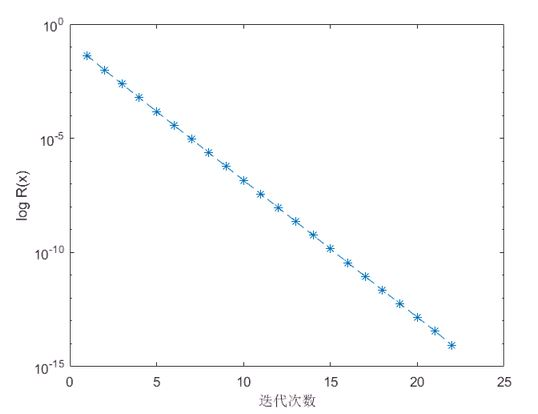
\includegraphics[width=0.5\textwidth]{T1a.JPG}
            \caption{自动控制误差的复化梯形积分误差随迭代次数变化的示意图}
        \end{figure}

    \item[$b)$] 参考教材125页的算法,定义目标精度$10^{-14}$,逐步计算$R(k,k)$,
                Matlab程序如下:
    \begin{lstlisting}[frame=single]
clear,clc
format long

%%参考课本125页算法
F = @(x) sin(cos(sin(cos(x)))); %积分函数
a = -1; b = 1;                  %积分区间[a,b]
e = 1e-14;                      %精度控制值
M=50;                           %最大循环次数
n=1;                            %迭代次数
h = b-a;
%%
I = zeros(M); %存储每一轮迭代计算得到的积分值,用于作图
%%step2
R = zeros(M,M);  %预置空间,用于存储R(0,0)~R(k,k)
R(1,1) = (F(a)+F(b))*h/2; %step2
I(1) = R(1,1);   %存储R(1,1)
%%step3,参考课本算法
for k = 2 : M
    hk = h/2^(k-1);
    R(k,1) = (R(k-1,1)+(2*hk)* sum(F(a + (2 * (1:2^(k-2)) - 1) * hk)))/2; 
    for j=2:k
        R(k,j) = R(k,j-1)+(R(k,j-1)-R(k-1,j -1))/(4^(j-1) -1);
    end
    I(k) = R(k,k); %存储每一轮得到的积分值
    n = n + 1;     %迭代次数+1
    if(abs(R(k,k )-R(k-1,k-1)) < e)
        RES = R(k,k) %step4,输出最终的积分值
        break;
    end
end
%%作图
fprintf('INF:迭代次数n=%d',n); %迭代次数
semilogy((1:n), abs(I(1:n)-RES), '-*');
xlabel('迭代次数');
ylabel('误差');
    \end{lstlisting}
        \quad \quad 程序输出:迭代次数$n=9$.计算可得分点数$=2^{9-1}=256$。
        最终积分结果$RES=1.339880713117284$.\\
        得到的误差图如下所示:
        \begin{figure}[h]
            \centering
            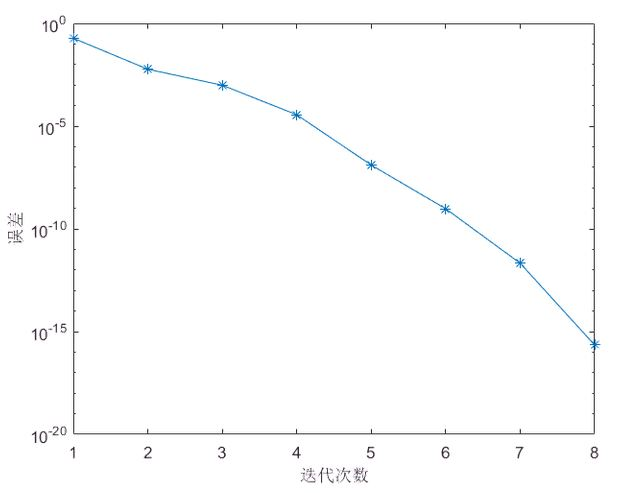
\includegraphics[width=0.8\textwidth]{T1b.JPG}
            \caption{龙贝格算法得到的积分误差随迭代次数变化的示意图}
        \end{figure}

    \item[$c)$] 高斯积分点和积分权重使用课程主页上的程序计算。
    \begin{lstlisting}[frame=single]
clear, clc

F = @(x) sin(cos(sin(cos(x)))); % 积分函数
a = -1; b = 1;                  % 积分区间[a,b]
e = 1e-14;                      % 精度控制
M = 50;                         %最大循环次数
I = zeros(M);    
  %预分配空间,用于存储每次计算得到的积分结果

[x, w] = gauss(1);   
  %调用课程主页函数,生成积分点和积分权重
I(1) = w * F(x);     %存储第一次迭代结果

for n = 2:M
    [x, w] = gauss(n);
    I(n) = w * F(x);
    if (abs(I(n) - I(n - 1)) < e)
        RES = I(n)   
            %输出最终的积分值,当作精确结果作误差图
        break;
    end  
end

fprintf('INF:迭代次数n=%d',n);    %迭代次数
semilogy((1:n), abs(I(1:n) - RES), '-*');
xlabel('迭代次数');
ylabel('Rx');

% GAUSS  nodes x (Legendre points) and weights w
%        for Gauss quadrature
function [x,w] = gauss(N)
  beta = .5./sqrt(1-(2*(1:N-1)).^(-2));
  T = diag(beta,1) + diag(beta,-1);
  [V,D] = eig(T);
  x = diag(D); [x,i] = sort(x);
  w = 2*V(1,i).^2;
end
    \end{lstlisting}
    \quad \quad 程序输出:迭代次数$n=14$.最终分点数$=n=14$。
    最终积分结果$RES=1.339880713117285$.\\
    得到的误差图如下所示:
        \\
        \\
        \\ 
        \\ 
    \begin{figure}[h]
        \centering
        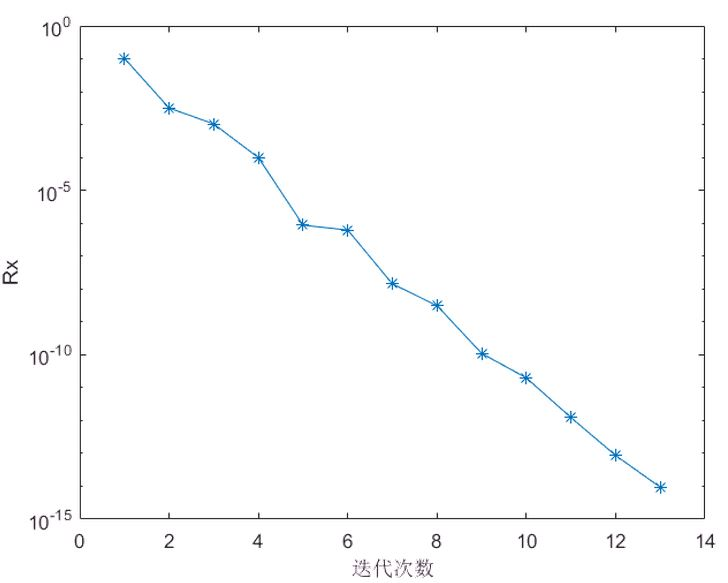
\includegraphics[width=0.8\textwidth]{T1C.JPG}
        \caption{高斯积分误差随迭代次数变化的示意图}
    \end{figure}

    \item[$d)$] 这三种算法在上述程序设计之下都将同一个积分结果运算到了$10^{-14}$级的精度,
                对它们的采样次数进行比较,是对总次数的比较。因此,结合上面得出的结果,复化
                梯形积分算法的总采样数为$1+2+4+···+2^{23}=2^{24}-1=16777215$次;龙贝格积分
                总的采样次数为$1+2+4+···+256=511$次;而高斯积分使用的采样点总数为$1+2+3+···+14=105$
                次。因此显然在达到相同的积分结果精度的情况下,复化梯形积分算法需要的积分点最多,开销最大,
                效率最低;龙贝格积分次之;而高斯积分能以较少的积分点数、采样点数完成同样精度的积分,在这
                三种算法中效率最高。

     
  \end{enumerate}
\item[第二题]
  \begin{enumerate}
    \item[$a)$] 即对拉格朗日插值基函数求导。由于分母对$x$是常数,仅考虑分子:
        \begin{eqnarray} 
            \left(\prod_{k=0,k\neq j}^{n}(x-x_k)\right)^{'} &=& [(x-x_0)(x-x_1)···(x-x_n)]^{'}\\
            &=& \prod_{k=1,k\neq j}^{n}(x-x_k)+(x-x_0)\left(\prod_{k=1,k\neq j}^{n}(x-x_k)\right)^{'}\\
            &=& \frac{\prod_{k=0,k\neq j}^{n}(x-x_k)}{x-x_0}+(x-x_0)\left(\prod_{k=1,k\neq j}^{n}(x-x_k)\right)^{'}\\
            &=& \frac{\prod_{k=0,k\neq j}^{n}(x-x_k)}{x-x_0}+ (x-x_0)\prod_{k=2,k\neq j}^{n}(x-x_k)\\
                &+& (x-x_0)\left(\prod_{k=2,k\neq j}^{n}(x-x_k)\right)^{'}   \nonumber\\
            &=& \frac{\prod_{k=0,k\neq j}^{n}(x-x_k)}{x-x_0}+ \frac{\prod_{k=0,k\neq j}^{n}(x-x_k)}{x-x_1}\\
                &+& (x-x_0)\left(\prod_{k=2,k\neq j}^{n}(x-x_k)\right)^{'}   \nonumber\\
            &=& ······· = \prod_{k=0,k\neq j}^{n}(x-x_k)\sum_{k=0,k\neq j}^{n}\frac{1}{x-x_k}
        \end{eqnarray}
        再考虑分母,两边同时除以分母$\pi_{j}$,立刻可得
        \begin{eqnarray} 
           &\ell_{j}^{'}(x)&=\ell_{j}(x)\sum_{k=0,k\neq j}^{n}(x-x_k)^{-1}\\
            \Longrightarrow &p^{'}(x)& = \sum_{j=0}^{n}f_{j}\ell_{j}^{'}(x) =
                         \sum_{j=0}^{n}\left(f_{j}\ell_{j}(x)\sum_{k=0,k\neq j}^{n}(x-x_k)^{-1}\right)    
        \end{eqnarray}

    \item[$b)$] 由题意即可写出matlab程序:
\begin{lstlisting}[frame=single]
    clear,clc,clf
LW = 'linewidth'; lw = 2;

F = @(x) sin(x); %原函数
f = @(x) cos(x); %标准导函数
n = 15;          %原函数插值点
m = 1000;        %误差检查点
xx = linspace(-1, 1, m+1);

y = zeros(1,1001);

for j = 1 : (m+1)
     y(j) = GETfx(-1,1,n,xx(j));
end

yy = f(xx);

Rx = abs(yy - y); %与真实解的误差绝对值

figure;
plot(xx, yy, 'k', LW, lw), hold on
plot(xx, y, 'b', LW, lw);
legend('真实值', '利用上题公式求出值');
xlabel('x');
ylabel('p(x)导数 or cos(x)');

figure;
semilogy(xx,Rx);
xlabel('x');
ylabel('Rx');

function fx = GETfx(a,b,n,x)
        %给定一点,输出插值求出的导数
    F = @(x) sin(x); %原函数
    ret = 0;
    inx = linspace(a, b, n + 1);
  for j = 1:n
    lx = 1;
    sum = 0; % 公式(1)中大括号内的求和部分
    
    for k = 1:j - 1
        lx = lx * (x - inx(k)) / (inx(j) - inx(k));
        sum = sum +1 / (x - inx(k));
    end
    %%避开k=j
    for k = j + 1:n
        lx = lx * (x - inx(k)) / (inx(j) - inx(k));
        sum = sum +1 / (x - inx(k));
    end
    ret = ret + F(inx(j)) * lx * sum;
  end    
    fx = ret;
end
\end{lstlisting}
        \quad \quad 得到的插值函数计算出的导数与精确值之间的图像:
        \begin{figure}[h]
            \centering
            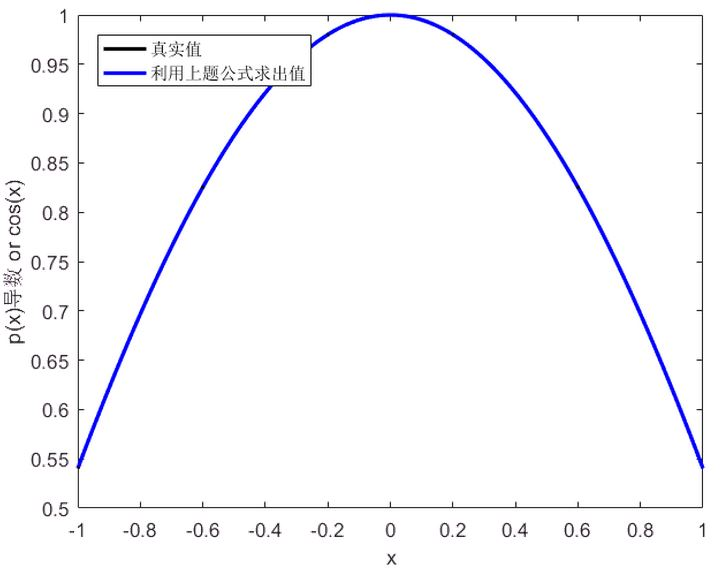
\includegraphics[width=0.7\textwidth]{T2B1.JPG}
            \caption{由插值函数计算出的导函数与精确值的函数示意图}
        \end{figure}\\
            得到的误差图如下所示:\\
            \\
            \\
        \begin{figure}[h]
              \centering
              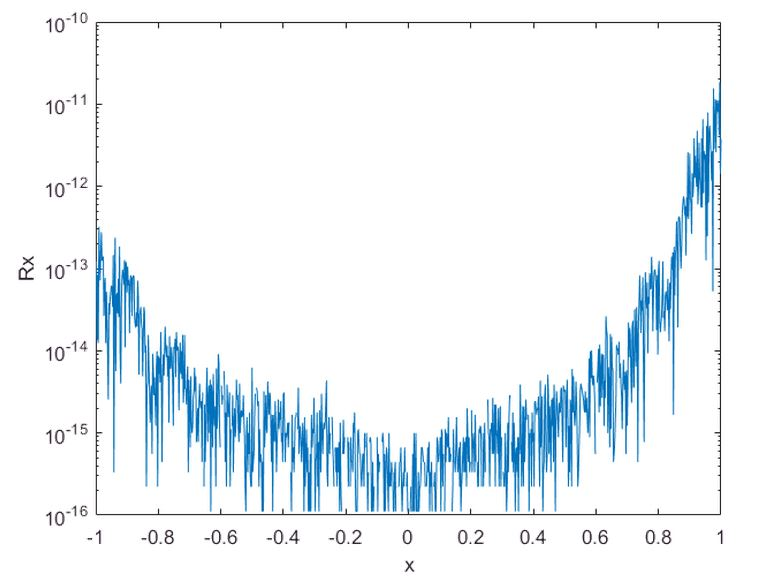
\includegraphics[width=0.7\textwidth]{T2B2.JPG}
              \caption{插值函数计算出的导函数与精确值之间的误差绝对值的示意图}
        \end{figure}

    \item[$c)$] 按给出的$p^{'}(x_i)$计算式,对任意$t\in[0,n]$,写出$p^{'}(x_t)$:
        \begin{eqnarray} 
            p^{'}(x_t)=\sum_{j=0}^{n}\left(f_{j}\ell_{j}(x_t)\sum_{k=0,k\neq j}^{n}(x_t-x_k)^{-1}\right)
        \end{eqnarray}
        以此来计算微分矩阵$D$中的第$t$行的元素,$p^{'}(x_t)=\sum_{j=0}^{n}f_{j}D_{tj}$:
        \begin{eqnarray} 
            D_{tj} &=& \ell_{j}(x_t)\sum_{k=0,k\neq j}^{n}(x_t-x_k)^{-1} = \frac{\prod_{m \neq j}(x_t-x_{m})}{\prod_{m \neq j}(x_{j}-x_{m})}\sum_{k=0,k\neq j}^{n}\frac{1}{(x_t-x_k)}\\
                   &=& \frac{1}{\pi_j}\sum_{k=0,k\neq j}^{n}\frac{\prod_{m \neq j}(x_t-x_{m})}{(x_t-x_k)}\\
                   &=& \frac{1}{\pi_j}\sum_{k=0,k\neq j}^{n}\prod_{m \neq j,k}(x_t-x_{m})\\
                   &=& \frac{1}{\pi_j}\prod_{m \neq j,t}(x_t-x_{m})\\
                   &=& \frac{\pi_t}{\pi_j(x_t-x_j)} \quad t\neq j
        \end{eqnarray}
        以上推导的 $(12)\Rightarrow (13)$ 步是因为$k\neq t$时,$\prod_{m \neq j,k}(x_t-x_{m})$都有一项$(x_t-x_t)$。\\
        特别的,当$t=j$时,可以更快得到简单推导出的表达式:
        \begin{eqnarray} 
            D_{tt}&=& \frac{\prod_{m \neq j}(x_t-x_{m})}{\prod_{m \neq j}(x_{j}-x_{m})}\sum_{k=0,k\neq j}^{n}\frac{1}{(x_t-x_k)} = \sum_{k=0,k\neq j}^{n}\frac{1}{(x_t-x_k)}\\
        \end{eqnarray}
        综上,根据第一小题推导出的结论,微分矩阵$D_{ij}$的元素可以表示为:
        \begin{equation}
            \label{eq6}
            D_{ij}=\left\{
            \begin{aligned}
                \frac{\pi_t}{\pi_j(x_t-x_j)}              & , & i\neq j \\
                \sum_{k=0,k\neq j}^{n}\frac{1}{(x_t-x_k)} & , & i=j.
            \end{aligned}
            \right.
        \end{equation}
        
        
    \item[$d)$] Matlab程序如下所示:
  \begin{lstlisting}[frame=single]
clear, clc, clf

F = @(x) sin(3 * x.^2);
dF = @(x) 6 * x .* cos(3 * x.^2);%定义原函数与导函数
max1 = zeros(1, 30);%总共30次计算,开辟30个空间
max2 = zeros(1, 30);%max1记录平均点,max2为切比雪夫点
nvec = (1:2:59);    %令n=1,3,5,...,57,59
j = 1;

for n = nvec        %对每一个n计算逐点误差的绝对值的最大值
    %等距点,以后缀1表示
    x1 = linspace(-1, 1, n + 1)';
    dp1 = diffM(x1) * F(x1);          %用微分矩阵计算的导数值
    max1(j) = max(abs(dp1 - dF(x1))); %误差绝对值最大值
    %切比雪夫点,以后缀2表示
    x2 = cos((0:n) * pi ./ n)';
    dp2 = diffM(x2) * F(x2);
    max2(j) = max(abs(dp2 - dF(x2)));
    %%
    j = j + 1;
end
%%由结果作图
plot1 = semilogy(nvec, max1, 'b-+'); hold on
plot2 = semilogy(nvec, max2, 'k-*');
xlabel('n');
ylabel('max Rx(n)');
legend([plot1, plot2], '等距点误差', '切比雪夫点误差');

function D = diffM(x)%%函数,生成微分矩阵D
n = length(x);
D = zeros(n, n);%输出结果为n*n的矩阵,初始化为0
PI = zeros(n); 
for i = 1:n     %预先将Πi全部计算出来并存储下来
    PI(i) = prod(x(i) - x((1:n) ~= i));
end
for i = 1:n  %双重循环生成矩阵
    for j = 1:n
        if (i ~= j)
            D(i, j) = PI(i) / (PI(j) * (x(i) - x(j)));
        else
            D(i, j) = sum(1 ./ (x(j) - x((1:n) ~= j)));
        end
    end
end
end
  \end{lstlisting}
        得到结果如下页图6所示。\\
        \begin{figure}[h]
            \centering
            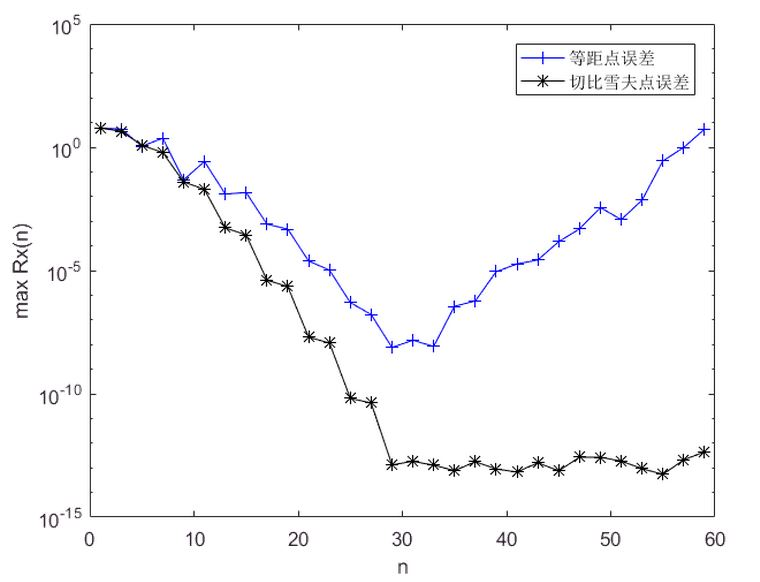
\includegraphics[width=0.6\textwidth]{T2D.JPG}
            \caption{取等距点和切比雪夫点产生的误差绝对值随n变化的示意图}
        \end{figure}
        \quad \quad 对比用等距点和切比雪夫点产生的误差,可以发现当$n$一直增大的过程中,若采用切比雪夫点则误差会
        快速下降到$10^{-14}~10^{-13}$左右,再增加分点对精度影响不大;而若采用等距点,则在$n$增大的
        过程中,误差先减小后面反而增大,在$n=29$附近达到误差极小值。采用等距点时误差随分点数增加而增
        大是因为产生了龙格现象,高阶多项式的插值效果反而不如低阶的。采用切比雪夫点插值则可以避免龙格
        现象的产生。
        \\
        \\
        \\

  \end{enumerate}


\item[第三题]
      \begin{enumerate}
        \item[$a)$] 观察右侧的形式,第一项为$y_{n-1}$,可知$p=1$;$f$有连续的四项,
                    可知$q=3$;而$f$的最高项为$f_{n+1}$,说明为隐式格式。\\
                        即推导$p=1,q=3$的隐式格式:\\
                        取$[x_{n-1},x_{n+1}]$为积分区间,以${x_{n+1},x_{n},x_{n-1},x_{n-2}}$
                    为积分节点,构造格式
                    \begin{eqnarray} 
                        y_{n+1}=y_{n-1}+h[\beta_0f_{n+1}+\beta_1f_{n}+\beta_2f_{n-1}+\beta_3f_{n-2}]
                    \end{eqnarray}
                    则由数值积分公式,有:
                    \begin{eqnarray} 
                        \beta_0h &=& \int_{x_{n-1}}^{x_{n+1}} 
                                    \frac{(x-x_{n})(x-x_{n-1})(x-x_{n-2})}{(x_{n+1}-x_n)(x_{n+1}-x_{n-1})(x_{n+1}-x_{n-2})} \mathrm{d}x \\
                                &=& \int_{t}^{t+2h} 
                                    \frac{(x-t-h)(x-t)(x-t+h)}{h\cdot 2h\cdot 3h} \mathrm{d}x  =  \frac{h}{3}  \nonumber\\ 
                        \beta_1h &=& \int_{x_{n-1}}^{x_{n+1}} 
                                    \frac{(x-x_{n+1})(x-x_{n-1})(x-x_{n-2})}{(x_{n}-x_{n+1})(x_{n}-x_{n-1})(x_{n}-x_{n-2})} \mathrm{d}x \\
                                &=& \int_{t}^{t+2h} 
                                    \frac{(x-t-2h)(x-t)(x-t+h)}{-h\cdot h\cdot 2h} \mathrm{d}x  =  \frac{4h}{3}  \nonumber\\ 
                        \beta_2h &=& \int_{x_{n-1}}^{x_{n+1}} 
                                    \frac{(x-x_{n+1})(x-x_{n})(x-x_{n-2})}{(x_{n-1}-x_{n+1})(x_{n-1}-x_{n})(x_{n-1}-x_{n-2})} \mathrm{d}x \\
                                &=& \int_{t}^{t+2h} 
                                    \frac{(x-t-2h)(x-t-h)(x-t+h)}{-2h\cdot -h\cdot h} \mathrm{d}x  =  \frac{h}{3}  \nonumber\\
                        \beta_3h &=& \int_{x_{n-1}}^{x_{n+1}} 
                                    \frac{(x-x_{n+1})(x-x_{n})(x-x_{n-1})}{(x_{n-2}-x_{n+1})(x_{n-2}-x_{n})(x_{n-2}-x_{n-1})} \mathrm{d}x \\
                                &=& \int_{t}^{t+2h} 
                                    \frac{(x-t-2h)(x-t-h)(x-t)}{-3h\cdot -2h\cdot -h} \mathrm{d}x  =  0  \nonumber 
                    \end{eqnarray}
                    得到格式:
                    \begin{eqnarray} 
                        y_{n+1}=y_{n-1}+\frac{h}{3}[f_{n+1}+4f_{n}+f_{n-1}]
                    \end{eqnarray}
        \item[$b)$] 计算其截断误差:
                    \begin{eqnarray} 
                        R(x) &=& \frac{y^{q+2}(\xi)}{(q+1)!}(x-x_n)(x-x_{n-1})···(x-x_{n-q}) \\
                        hT_{n+1} &=& \int_{x_{n-p}}^{x_{n+1}}R(x)\mathrm{d}x \\
                                 &=& \int_{x_{n-1}}^{x_{n+1}}\frac{y^{5}(\xi)}{24}(x-x_n)(x-x_{n-1})(x-x_{n-2})(x-x_{n-3})\mathrm{d}x\\
                                 &=& \frac{29h^{5}y^{5}(\xi)}{90}
                    \end{eqnarray}
                    这是四阶格式。
        \item[$c)$] 使用三阶龙格-库塔方法起步,由于恰好计算格式中$f_{n-2}$系数为0,可以从第三项
                    开始使用线性多步法,因此只需起步前两项。Matlab程序如下:
                \begin{lstlisting}[frame=single]
clear, clc, clf
format long

%%
a = 0; b = 2;               %求解区间[0, 2]
n = 1000;                   %取样点数
h = (b - a) / n;            %步长
x = linspace(a, b, n+1)';   %取样点
EXCY = @(x) x.^2.*exp(-5.*x)./2; %解析解
yn = zeros(n+1, 1); %存储函数在取样点处的数值解
yn(1) = 0;          %初值条件
f = @(x, y) x * exp(-5 * x) - 5 * y;
%%使用三阶龙格-库塔方法起步前两项
    k1 = f(x(1), yn(1));
    k2 = f(x(1) + h / 2, yn(1) + (h / 2) * k1 );
    k3 = f(x(1) + h, yn(1) - h * k1 + 2 * h * k2 );
    yn(2) = yn(1) + (h / 6) * (k1 + 4 * k2 + k3);


%% 使用4阶的线性多步法从第3项开始计算
g = x .* exp(-5 .* x); %简化表达
for i = 2:n
    yn(i + 1) = (yn(i - 1) + (h / 3) * (g(i - 1) - 5 * yn(i - 1) + 4 * g(i) - 20 * yn(i) + g(i + 1))) / (1 + 5 * h / 3);
end

EXY = EXCY(x); % 解析解在取样点处的取值

pic1 = plot(x, yn, 'k'); hold on
pic2 = plot(x, EXY, 'b');
legend([pic1, pic2], '数值解', '解析解');
xlabel('x');
ylabel('y');
                \end{lstlisting}
                得到的解的图像与解析解的图像如下图所示:\\
                \begin{figure}[h]
                    \centering
                    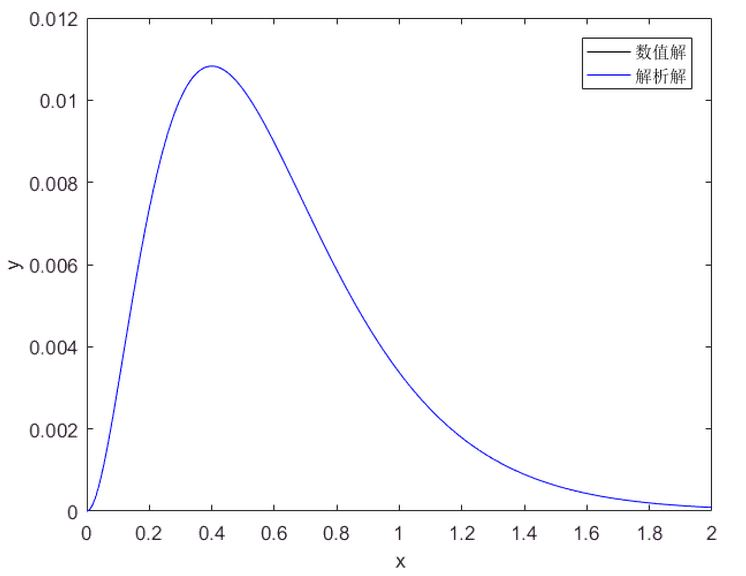
\includegraphics[width=0.6\textwidth]{T3C.JPG}
                    \caption{利用三阶龙格-库塔方法起步的线性多步法求解出的函数示意图}
                \end{figure}\\
                \quad \quad 三阶龙格-库塔方法是三阶精度的计算公式,上面推导出的四步四阶线性多步法是四阶
                精度的计算公式。因此满足“起步格式的精度至多只能比该格式的精度低一阶”的条件,
                不影响格式的整体误差。
                \\
                

        \item[$d)$] 推导这个一阶线性常微分方程的解,直接利用通解公式\\
                    此时$P(x)=5,Q(x)=xe^{-5x}$:
                    \begin{eqnarray} 
                        y &=& Ce^{-\int P(x)\mathrm{d}x}+e^{-\int P(x)\mathrm{d}x}\int Q(x)e^{\int P(x)\mathrm{d}x}\mathrm{d}x\\
                          &=& Ce^{-5x}+e^{-5x}\int xe^{-5x}e^{5x}\mathrm{d}x\\
                          &=& Ce^{-5x}+\frac{x^{2}e^{-5x}}{2}
                    \end{eqnarray}
                    再代入边界条件$y(0)=0$,立即得到$C=0$。则解为:
                    \begin{eqnarray} 
                        y = \frac{x^2e^{-5x}}{2}
                    \end{eqnarray}
                    这就是上述方程的精确解。\\
                    要验证推断的阶数是否正确,可以从误差随h增长的变化速度中看出来。

            \begin{lstlisting}[frame=single]
clear, clc, clf

a = 0; b = 2; % 求解区间[0, 2]
y = @(x) (x.^2) .* exp(-5 .* x) / 2; %精确解
f = @(x, y) x * exp(-5 * x) - 5 * y; %导数
nvec = 50:500;            % 取样点数
hvec = (b - a) ./ (nvec); %步长变化,用于作图
maxe = zeros(length(nvec), 1)';
iteration = 1;            %计数

for n = nvec              %对n迭代
    h = (b - a) / (n);        %步长
    x = linspace(a, b, n+1)'; % 取样点
    
    yn = zeros(n+1, 1); %存储计算出的函数在取样点处的数值解
    yn(1) = 0;          %初值条件

%%使用三阶龙格-库塔方法起步前两项
    k1 = f(x(1), yn(1));
    k2 = f(x(1) + h / 2, yn(1) + (h / 2) * k1 );
    k3 = f(x(1) + h, yn(1) - h * k1 + 2 * h * k2 );
    yn(2) = yn(1) + (h / 6) * (k1 + 4 * k2 + k3);   
%% 使用4阶的线性多步法从第3项开始计算
    g = x .* exp(-5 .* x); %简化表达
    for i = 3:n - 1
        yn(i + 1) = (yn(i - 1) + (h / 3) * (g(i - 1) - 5 * yn(i - 1) + 4 * g(i) - 20 * yn(i) + g(i + 1))) / (1 + 5 * h / 3);
    end
    YE = y(x); % 精确解在取样点处的取值
    maxe(iteration) = max(abs(YE - yn));%记录当前n中最大的误差
    iteration = iteration + 1;
end
%%作出最大误差随n变化的loglog图
loglog(hvec, maxe, 'k'); hold on
xlabel('h')
ylabel('max Rn(x)')
            \end{lstlisting}
            程序的运行结果如下所示:\\
            \begin{figure}[h]
                \centering
                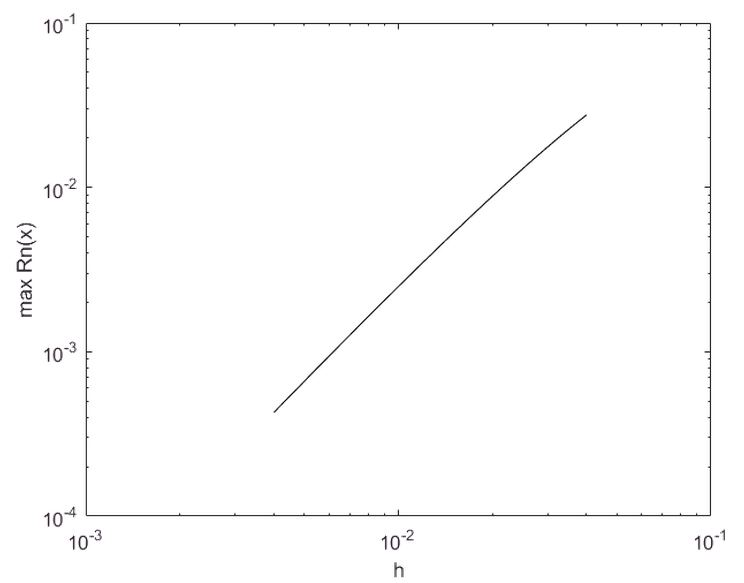
\includegraphics[width=0.6\textwidth]{T3D.JPG}
                \caption{误差随h增长的loglog示意图}
            \end{figure}\\
            图中loglog线的斜率代表计算精度。

       \end{enumerate}



\end{enumerate}




\end{document}
